%==================================================================================
%==================================================================================
% Document		:		Chapitre: Approche statistique pour le résumé automatique de textes
%
% Auteur		: 		Abdelkrime ARIES
% Encadreur		:		Dr. Omar NOUALI
% Co-encadreur	:		Mme. Houda OUFAIDA
% Établissement	:		ESI (Ecole Nationale Supérieure d'Informatique; ex. INI) 
% Adresse		:		Oued Smar, Alger, Algérie 
% Année			:		2012/2013
% Grade			:		Magister
% Discipline 	:		Informatique 
% Spécialité	:		IRM (Informatique Répartie et Mobile)
% Titre			:		Résumé automatique de textes
%
%==================================================================================
%==================================================================================

%==========================L'entete de chapitre====================================
%==================================================================================
 \ifx\wholebook\relax\else
  	\documentclass[a4paper,12pt,oneside]{../use/ESIthesis}
  	
  	\usepackage{amsmath,amssymb}             % AMS Math
\usepackage[utf8]{inputenc}
%\usepackage[T1]{fontenc} %,LAE 
\usepackage[T1]{fontenc}
%\usepackage[french,english]{babel}
\usepackage[frenchb]{babel}
\usepackage{microtype}

%\usepackage[left=2.5cm,right=2.5cm,top=2.5cm,bottom=2.5cm,includefoot,includehead,headheight=13.6pt]{geometry}
\usepackage[left=2.8cm,right=2.2cm,top=2.8cm,bottom=2.8cm,includefoot,includehead,headheight=13.6pt]{geometry}
%\usepackage[left=3.8cm,right=3.2cm,top=2.8cm,bottom=2.8cm,includefoot,includehead,headheight=13.6pt]{geometry}
%\usepackage[left=1.5in,right=1.3in,top=1.1in,bottom=1.1in,includefoot,includehead,headheight=13.6pt]{geometry}
\renewcommand{\baselinestretch}{1.5}

% Table of contents for each chapter

\usepackage[nottoc, notlof, notlot]{tocbibind}
\usepackage[french]{minitoc}
\setcounter{minitocdepth}{1}
\mtcindent=15pt
% Use \minitoc where to put a table of contents

\usepackage{aecompl}

% Glossary / list of abbreviations

\usepackage[intoc]{nomencl}
%\renewcommand{\nomname}{List of Abbreviations}

\makenomenclature

% My pdf code

\usepackage[pdftex]{graphicx}
\usepackage[a4paper,pagebackref,hyperindex=true]{hyperref}

%I added
%\usepackage{tabulary}
%\usepackage{longtable}
%\usepackage[table]{xcolor}
\usepackage{indentfirst}


% Links in pdf
\usepackage{color}
%\definecolor{linkcol}{rgb}{0,0,0.4} 
%\definecolor{citecol}{rgb}{0.5,0,0} 

% Change this to change the informations included in the pdf file

% See hyperref documentation for information on those parameters

\hypersetup
{
%bookmarksopen=true,
pdftitle=Résumé Automatique de Textes,
pdfauthor=Abdelkrime ARIES, 
pdfsubject= {Résumé automatique de textes en utilisant une approche statistique, le regroupement, et la classification} , %subject of the document
%%pdftoolbar=false, % toolbar hidden
%pdfmenubar=true, %menubar shown
%pdfhighlight=/O, %effect of clicking on a link
colorlinks=false, %couleurs sur les liens hypertextes
%pdfpagemode=None, %aucun mode de page
%pdfpagelayout=SinglePage, %ouverture en simple page
%pdffitwindow=true, %pages ouvertes entierement dans toute la fenetre
%linkcolor=linkcol, %couleur des liens hypertextes internes
%citecolor=citecol, %couleur des liens pour les citations
%urlcolor=linkcol %couleur des liens pour les url
}



% Some useful commands and shortcut for maths:  partial derivative and stuff

\newcommand{\pd}[2]{\frac{\partial #1}{\partial #2}}
\def\abs{\operatorname{abs}}
\def\argmax{\operatornamewithlimits{arg\,max}}
\def\argmin{\operatornamewithlimits{arg\,min}}
\def\diag{\operatorname{Diag}}
\newcommand{\eqRef}[1]{(\ref{#1})}

\usepackage{rotating}                    % Sideways of figures & tables
%\usepackage{bibunits}
%\usepackage[sectionbib]{chapterbib}          % Cross-reference package (Natural BiB)
%\usepackage{natbib}                  % Put References at the end of each chapter
                                         % Do not put 'sectionbib' option here.
                                         % Sectionbib option in 'natbib' will do.
\usepackage{fancyhdr}                    % Fancy Header and Footer

\usepackage{txfonts}                     % Public Times New Roman text & math font
  
%%% Fancy Header %%%%%%%%%%%%%%%%%%%%%%%%%%%%%%%%%%%%%%%%%%%%%%%%%%%%%%%%%%%%%%%%%%
% Fancy Header Style Options

\pagestyle{fancy}                       % Sets fancy header and footer
\fancyfoot{}                            % Delete current footer settings

%\renewcommand{\chaptermark}[1]{         % Lower Case Chapter marker style
%  \markboth{\chaptername\ \thechapter.\ #1}}{}} %

%\renewcommand{\sectionmark}[1]{         % Lower case Section marker style
%  \markright{\thesection.\ #1}}         %
%\fancyhead[LE,RO]{\bfseries\thepage}    % Page number (boldface) in left on even
%										% pages and right on odd pages
%\fancyhead[RE]{\bfseries\nouppercase{\leftmark}}      % Chapter in the right on even pages
%\fancyhead[LO]{\bfseries\nouppercase{\rightmark}}     % Section in the left on odd pages

\fancyhead[R]{\bfseries\thepage}    % Page number (boldface) in right
\fancyhead[L]{\bfseries\nouppercase{\rightmark}}     % Section in the left on odd pages

\let\headruleORIG\headrule
\renewcommand{\headrule}{\color{black} \headruleORIG}
\renewcommand{\headrulewidth}{1.0pt}
\usepackage{colortbl}
\arrayrulecolor{black}

\fancypagestyle{plain}{
  \fancyhead{}
  \fancyfoot{}
  \renewcommand{\headrulewidth}{0pt}
}

%\usepackage{algorithm}
%\usepackage[noend]{algorithmic}

%%% Clear Header %%%%%%%%%%%%%%%%%%%%%%%%%%%%%%%%%%%%%%%%%%%%%%%%%%%%%%%%%%%%%%%%%%
% Clear Header Style on the Last Empty Odd pages
\makeatletter

\def\cleardoublepage{\clearpage\if@twoside \ifodd\c@page\else%
  \hbox{}%
  \thispagestyle{empty}%              % Empty header styles
  \newpage%
  \if@twocolumn\hbox{}\newpage\fi\fi\fi}

\makeatother
 
%%%%%%%%%%%%%%%%%%%%%%%%%%%%%%%%%%%%%%%%%%%%%%%%%%%%%%%%%%%%%%%%%%%%%%%%%%%%%%% 
% Prints your review date and 'Draft Version' (From Josullvn, CS, CMU)
\newcommand{\reviewtimetoday}[2]{\special{!userdict begin
    /bop-hook{gsave 20 710 translate 45 rotate 0.8 setgray
      /Times-Roman findfont 12 scalefont setfont 0 0   moveto (#1) show
      0 -12 moveto (#2) show grestore}def end}}
% You can turn on or off this option.
% \reviewtimetoday{\today}{Draft Version}
%%%%%%%%%%%%%%%%%%%%%%%%%%%%%%%%%%%%%%%%%%%%%%%%%%%%%%%%%%%%%%%%%%%%%%%%%%%%%%% 

\newenvironment{maxime}[1]
{
\vspace*{0cm}
\hfill
\begin{minipage}{0.5\textwidth}%
%\rule[0.5ex]{\textwidth}{0.1mm}\\%
\hrulefill $\:$ {\bf #1}\\
%\vspace*{-0.25cm}
\it 
}%
{%

\hrulefill
\vspace*{0.5cm}%
\end{minipage}
}

\let\minitocORIG\minitoc
\renewcommand{\minitoc}{\minitocORIG \vspace{1.5em}} %1.5em

\usepackage{multirow}
%\usepackage{slashbox}

\newenvironment{bulletList}%
{ \begin{list}%
	{$\bullet$}%
	{\setlength{\labelwidth}{25pt}%
	 \setlength{\leftmargin}{30pt}%
	 \setlength{\itemsep}{\parsep}}}%
{ \end{list} }

\newtheorem{definition}{Définition }
\renewcommand{\epsilon}{\varepsilon}

% centered page environment

\newenvironment{vcenterpage}
{\newpage\vspace*{\fill}\thispagestyle{empty}\renewcommand{\headrulewidth}{0pt}}
{\vspace*{\fill}}

%%%%%%%%%%%%%%%%%%%%%%%%%%%%%%%%%%%%%%%%%%%%%%%%%%%%%%%%%%%%%%%%%%%%
% Par Karim
%%%%%%%%%%%%%%%%%%%%%%%%%%%%%%%%%%%%%%%%%%%%%%%%%%%%%%%%%%%%%%%%%%%%
%for the degree sign
\usepackage{textcomp} 
\usepackage{bookmark}
\usepackage{framed}
\usepackage{arabtex}
%\usepackage{nashbf}
%\usepackage{atrans}
%calligra font for the remerciement
\usepackage{calligra}

%List of acronyms
\usepackage{acronym}

\newcommand{\racine}{./}

\newcommand{\setracine}[1]{\renewcommand{\racine}{#1}}

\newcommand{\tablefile}[1]{\input{\racine tab/#1}}
\newcommand{\appendixfile}[1]{\input{\racine anx/#1}}
%\newcommand{\chapterfile}[1]{\input{\racine chap/#1}}

\newcommand{\stitle}[1]{
\noindent
\textbf{#1}
}

\newenvironment{itemizeb}
{\begin{list}{\textbullet} {\setlength{\rightmargin}{0cm} \setlength{\leftmargin}{1cm}}}
{\end{list}}


\newenvironment{itemizec}
{\begin{list}{\textopenbullet} {\setlength{\rightmargin}{0cm} \setlength{\leftmargin}{1cm}}}
{\end{list}}


\newcommand{\kexpbox}[1]{

\vspace{5mm}
\noindent
 \fbox{%
   \parbox{0.985\linewidth}{%
   \vspace{2mm}
   {\large  \textbf{Exemple:}}\\
      #1
   }%
 }
}

\newcommand{\kbox}[1]{

\vspace{2mm}
\noindent
 \fbox{%
   \parbox{0.965\linewidth}{%
   \vspace{2mm}
      #1
   }%
 }
}

\newenvironment{kexp}
{
\begin{framed}
\noindent
{\large  \textbf{Exemple:}}\\
}
{
\end{framed}
}

%%%%%%%%%%%%%%%%%%%%%%%%%%%%%%%%%%%%%%%%%%%%%%%%%%%%%%%%%%%%%%%%%%%%
%%%%%%%%%%%%%%%%%%%%%%%%%%%%%%%%%%%%%%%%%%%%%%%%%%%%%%%%%%%%%%%%%%%%

% definitions.
% -------------------

\setcounter{secnumdepth}{3}
\setcounter{tocdepth}{2}

\newcommand{\tab}[1]{{\hskip #1}}
  	 	
  	 	\setracine{../}
  	 	\graphicspath{{.}{../fig/}}
  	 	
  	 	\begin{document}
  	 	
  	 	\dominitoc 
  	 	\selectlanguage {francais}
  	 	%just to create the .toc file, then you can hide it
  	 	%\tableofcontents
  	 	\mainmatter
  \fi
%==================================================================================

\chapter{Approche statistique pour le résumé automatique de textes}
\label{chap:RATstat}
\minitoc

\section{Introduction}

L'approche statistique se caractérise par sa "simple" mise en œuvre, sa robustesse, et son indépendance vis-à-vis le domaine, si on la compare à l'approche linguistique. 
Elle nous apparut très intéressante et prometteuse, étant donné que les outils de recherche de l'information sont en constante évolution. 
L'approche statistique utilise différents critères pour calculer le score de l'unité qu'on veut extraire. 
Ces critères sont combinés de différentes manières afin de procéder à un score qu'on peut utiliser pour juger si l'unité peut être retenue dans le résumé. 
%Avant de calculer le score, il faut d'abord faire un pré-traitement sur le texte d'entrée. 
Ceci nécessite d'effectuer un pré-traitement du texte source.
Les résumés issus de cette approche présentent des inconvénients comme les anaphores, manque de cohérence et cohésion.
Pour diminuer ces limites, une étape de post-traitement est nécessaire. 

Dans ce chapitre, nous allons aborder le travail de Luhn, qui va nous aider à comprendre cette méthode et même les problèmes du résumé automatique. 
Ensuite, comme tout système de RI ou de TALN, ceci nécessite une étape de pré-traitement qui nous garde que l'information pertinente dont le système a besoin. 
Ainsi que les critères fondamentaux pour le calcul du score d'une unité du texte, quelques exemples sur le calcul de score sont ensuite présentés. 
Les scores de ces critères vont être combinées pour avoir un seul score qui nous aide à juger la pertinence d'une unité (en général: phrase), pour ceci nous allons présenter comment peut-on combiner ces différents scores. 
Après, nous allons discuter quelques méthodes utilisées pour améliorer l'approche statistique. 
Enfin, nous allons présenter des méthodes pour améliorer la structure et la lisibilité du résumé résultant, dans la section post-traitement. 
Dans la suite de ce chapitre nous allons utiliser la phrase comme unité d'extraction, à moins qu'il y a des recherches qui prend une autre unité.

\section{Travail de Luhn}

Le travail de Luhn \cite{58-luhn} est considéré comme le premier travail dans le domaine de résumé automatique. 
La plupart des systèmes de résumé actuels s'inspirent de ce travail. 
Luhn, dans son travail, utilise la fréquence de mots (voir la section \ref{sec:crit-stat}) ainsi que la position des mots dans la phrase, pour calculer l'importance d'une phrase. 
Dans ce qui suit, nous allons présenter les étapes de résumé comme proposé par Luhn, dont le pré-traitement et le calcul des scores de phrases.
Ces étapes sont, ensuite, reprises et étendues dans les systèmes de RA statistiques.

\subsection{Pré-traitement}

%TODO segmentation: Luhn
% *H. P. Luhn, “A Statistical Approach to Mechanized Encoding and Searching of Literary Information,”
% IBM Journal of Research and Development , 1, No. 4, 309-317(October1957).

Luhn utilise un algorithme simple de radicalisation (voir la section \ref{sec:pre-trait}), pour avoir le radical d'un mot. 
Par exemple, les mots "\textit{differ}", "\textit{differentiate}", "\textit{different}", "\textit{differently}","\textit{difference}", et "\textit{differential}" ont le même radical. 
Le principe est d'assembler les mots qui se prononcent de la même manière au début en commençant par le premier caractères. 
Les mots sont comparée deux-à-deux, lorsque on atteint le premier échec, on commence à compter le nombre des caractères restants. 
Si le nombre des caractères restants est inférieur ou égale à six, les deux mots sont jugés similaires. 

%Stop words removal
Pour les mots communs, ils sont des mots qui se répètent dans tous les documents comme les prépositions, etc. et qui n'ajoute rien en terme d'information, leur fonction est de faire la liaison entre les mots sensibles. 
Pour éviter que ces mots biaisent le score de phrases, Luhn propose la suppression de ces mots appelés mots vides. 
Pour ce faire, Luhn utilise une liste des mots communs préparée manuellement à comparer aux mots du texte d'entrée. 

\subsection{Calcul du score}

Pour extraire les phrases pertinentes, il est nécessaire d'attribuer à chaque phrase un score reflétant son importance. 
Luhn utilise une méthode où le score est calculé en fonction de fréquences des mots et leurs positions dans la phrase. 
Dans le contexte des articles scientifiques, ce choix est motivé par:
\begin{itemize}
\item L'auteur répète les mots importants dans l'article. 
\item Plus que certains mots sont accompagnés avec d'autres dans une phrase, plus son importance augmente. 
\item Il est peu possible qu'un mot peut refléter plus qu'une notion. 
\item Il est peu possible que l'auteur utilise différents mots pour refléter la même notion. 
\end{itemize}

%Donc, Luhn a suivi une procédure pour calculer le score des phrases et générer le résumé en utilisant les fréquences des mots et leurs positions dans la phrase. 
%La procédure peut être résumée dans les points suivants:
La méthode proposée peut être résumée dans les points suivants:
\begin{enumerate}
\item Calculer la fréquence de mots non vides. 
\item Les mots signifiants sont ceux qui ont des fréquences comprises entre deux seuils prédéfinis. 
\item Pour chaque phrase, on définit un groupe qui contient les mots signifiants ayant une distance de 5 à 6 mots non signifiants entre eux. 
\item Si une phrase contient plus d'un groupe, on choisit celui contenant plus de mots signifiants. 
\item Pour calculer le score de la phrase, soit $ S $ le nombre de mots signifiants, et $ T $ est le nombre total des mots dans ce groupe. 
Le score va être $ \frac{S^2}{T} $. 
Un exemple est donné dans la figure \ref{fig:luhn-score}, où $ S = 4 $ et $ T = 7 $ ce qui nous donne un score de $ \frac{4^2}{7} \approx 2.3  $.
\item Les phrases ayant un score supérieur à certain seuil sont sélectionnées. 
\end{enumerate}

\begin{figure}[ht]
\begin{center}
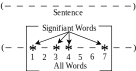
\includegraphics{RATstat/luhn-score.pdf} % % %[width=140mm]
 \caption[Score d'une phrase selon Luhn]{Score d'une phrase selon Luhn \cite{58-luhn}.}
 \label{fig:luhn-score}
\end{center}
\end{figure}

\section{Pré-traitement}
\label{sec:pre-trait}

%Resource Lean and Portable Automatic Text Summarization page 24 \\
Le pré-traitement dans le résumé automatique de textes (ou la recherche d'information en général) est une tâche très importante, liée à la langue traitée. 
En discutant le travail de Luhn, nous avons introduit les différentes étapes utilisées dans le pré-traitement. 
%Nous avons vu son importance en discutant le travail de Luhn.
Ces étapes étant la normalisation, la segmentation, la radicalisation, la suppression de mots vides, etc., sont des techniques du TALN \cite{04-brants}. 
Elles sont utilisées par les systèmes de résumé automatique afin de rendre le texte d'entrée plus facile à traiter et de le transformer à un standard qui est utilisé comme entrée au module de traitement. 
%Natural Language Processing in Information Retrieval.pdf

\subsection{Normalisation}

 %Church, K.: One Term or Two? In: Proceedings of SIGIR 1995, pp. 310–318 (1995)
La normalisation est la procédure qui transforme un document dans un format standard plus facile à manipuler. 
Par exemple, un document peut contenir les mots équivalents "Mr.", "Mr", "mister", et "Mister", qui peuvent tous être normalisés en un seul mot. 

%Un des algorithmes pour la normalisation de la langue Arabe est celui de [Larkey et al., 2002], procédé comme suite: 
Parmi les opérations effectuées dans cette étape:
\begin{itemize}
\item Suppression des caractères spéciaux et des chiffres. 
\item Remplacement de certains mots équivalents, comme les abréviations (voir l'exemple précédent). 
\item Dans certaines langues comme la langue Arabe, élimination des diacritiques. 
\item Remplacement de certains caractères, comme l'algorithme de \cite{02-larkey-al} destiné à diminuer les variations qui peuvent exister lors de l'écriture d'un mot en arabe. 
\item La suppression de certaines formes de style, comme celles des pages Web. 
\end{itemize}
La radicalisation est aussi une forme de normalisation, elle sera discutée ultérieurement (voir la section \ref{sec:stemming}).

\subsection{Segmentation}

Dans le résumé par extraction, il est nécessaire de décider sur quelle granularité nos segments vont être extraits, c.-à-d.  la taille de chaque unité extraite pour former le résumé. 
Elle peut être un paragraphe, une phrase, ou une clause; bien que dans la plupart des cas, l'extraction se fait au niveau de phrase. 
Dans l'approche statistique, les traitements sont exécutés sur les mots qui doivent être segmentés eux aussi, on appelle ça en anglais: Tokenization. 

\subsubsection{Segmentation du texte en phrases}

%La détection des limites en utilisant la ponctuation et le contexte
Dans la plupart des langues écrites, les phrases sont délimitées par des marques de ponctuation comme le point, le point d'exclamation, le point d'interrogation. 
La phrase est définie par une clause qui commence par une lettre majuscule et se termine par un des trois marques de ponctuation précédentes \cite{90-nunberg}. 
Mais, il existe des cas où cette définition ne peut pas être appliquée: 
\begin{itemize}
\item Le point peut être utilisé dans les abréviations, par exemple "Mr.", "Dr.", "etc.", etc., qui se trouvent dans la plupart des cas au milieu d'une phrase. 
\item Les phrases peuvent être délimitées par plusieurs autres marques de ponctuation \cite{10-palmer}. 
Il existe des cas où des phrases sont délimitées par des marques autres que les points, comme par exemple les virgules utilisées par les séquences d'actions. 
\item Dans des langues, comme le Thaï, il n'existe pas de ponctuation pour différencier les limites de phrases. 
\end{itemize}

Plusieurs facteurs contextuels ont été proposés pour aider à la segmentation en phrases, comme \cite{10-palmer}:
\begin{itemize}
\item Distinction de la casse: les mots commençant par une lettre majuscule donnent une information sur les limites de phrases. 
Les phrases commencent toujours par une lettre en majuscule.

\item Parties du discours (Part of speech): \cite{97-palmer-hearst} ont prouvé que l'utilisation des parties de discours qui entourent une marque de ponctuation avec un algorithme d'apprentissage, peuvent aider à détecter les limites de phrases. 

\item Longueur du mot: La longueur de mots avant et après un point, est utilisée par \cite{89-riley}, comme un critère contextuel. 

\item Les suffixes: \cite{80-muller-al} utilisent l'analyse morphologique pour identifier les suffixes, et de ce fait filtrer les mots qui ne sont pas des abréviations. 
Ceci est utilisé pour identifier les mots qui ne figurent pas dans la liste des abréviations. 

\item Préfixes et suffixes: \cite{97-reynar-ratnaparkhi} utilisent les préfixes et les suffixes des mots entourant la marque de ponctuation, comme un critère contextuel. 
\item Les classes des abréviations: \cite{89-riley} et \cite{97-reynar-ratnaparkhi} divisent les abréviations sur des catégories comme les titres (qui ne peuvent pas être à la fin de phrase, comme \textit{Mr.}, \textit{Dr.}, etc.) et les indicatifs corporatifs (qui peuvent être à la fin de phrase, comme \textit{Corp.}, \textit{S.p.A.}, etc.). 

\item Les noms propres: \cite{02-mikheev} utilise la présence des noms propres à droite du point comme critère. 
\end{itemize}

%Les différents algorithmes de détection de limites
Pour détecter les limites de phrases, il existe deux approches: l'approche basée sur les règles manuelles, et l'approche par apprentissage. 
La première approche est la plus ancienne et la plus utilisée \cite{10-palmer} parmi ces deux approches, pour déterminer les limites de phrases. 
Elle utilise une grammaire régulière définie manuellement, avec une liste des abréviations et des noms propres. 
Un des algorithmes basés sur les expressions régulières, est le système d'extraction de l'information \textit{Alembic} développé par \cite{95-aberdeen-al}. 
Il contient des différents modules qui tentent de classifier toute sorte de marque de ponctuation en identifiant le point dans les nombres, les expressions de date et de temps, et les abréviations. 
Il utilise une liste de 75 abréviations et une série de plus de 100 règles manuelles. 
Cette approche est développée pour un corpus et une langue spécifique et se base sur les listes de mots spécifiques pour une langue.
Ainsi, pour l'appliquer sur une autre langue il faut les redéfinir à nouveau. 

La première approche requiert un grand effort pour écrire les règles de détection les délimiteurs et la préparation de la liste des abréviations. 
Les méthodes par apprentissage tentent de définir ces règles de manière automatique, ceci permettra de varier les langues, les applications, et les genres. 
Le premier travail utilisant cette approche pour la segmentation en phrases, est celui de \cite{89-riley}. 
Sa méthode utilise les arbres de régression \cite{84-breiman-al} pour classifier les points selon des critères contextuels concernant les mots qui précèdent et qui suivent les points. 
Ces critères contextuels comportent: la longueur du mot, la ponctuation après le point, les classes d'abréviation, la casse du mot, et la probabilité que le mot ayant place au début ou à la fin de la phrase. 
Les algorithmes basant sur l'approche par apprentissage, sont nécessaires pour fournir des traitements robustes sur une variété de textes et de langues. 

\subsubsection{Segmentation du texte en mots (Tokenization)}

La segmentation de mots est une étape nécessaire pour exécuter les traitements statistiques. 
Dans la plupart de systèmes d'écriture, les mots sont séparés par des espaces. 
Un simple algorithme de segmentation de mots considère tous les caractères consécutifs précédés et suivis par un espace, comme un mot. 
Cette convention est sujet de plusieurs problèmes:
%
\begin{itemize}
%
\item Les marques de ponctuation sont considérées comme un terme séparé. 
Mais dans le cas du point, on peut trouver qu'il peut être attaché à un autre terme, comme les abréviations qui se terminent toujours par un point. 
%
\item Les marques de citation (\textquotedblleft \textquotedblright \textquoteleft \textquoteright) sont utilisées pour spécifier le début et la fin d'une citation. 
Les guillemets de citation et l'apostrophe ont le même caractère, et donc on ne peut pas déterminer immédiatement si la marque est un guillemet ou une apostrophe. 
%
\item L'apostrophe est une source d'ambiguïté dans la segmentation de mots. 
Dans l'anglais, l'apostrophe peut être utilisée avec un "\textit{s}" dans la forme possessive (\textit{Karim's thesis}), dans la contraction du verbe "\textit{is}" (\textit{she's}, \textit{it's}, etc.), comme elle peut être utilisée dans le pluriel de certains mots (\textit{I.D.'s}, \textit{1980's}, etc.). 
L'apostrophe est aussi utilisée dans les cas de contraction. 
Dans l'anglais, les contractions "\textit{I'm}" et "\textit{we've}" sont segmentés comme "\textit{I am}" et "\textit{we have}" respectivement. 
Pour le français, on peut citer un ensemble de contractions, y compris: la contraction des articles (\textit{l'homme}, \textit{c'était}), la contraction des pronoms (\textit{j'ai}, \textit{je l'ai}), et autres formes (\textit{n'y}, \textit{qu'ils}, \textit{d'ailleurs}).
%
\item Certaines langues contiennent des mots composés, soit en attachant un mot à l'autre, soit par trait d'union. 
Dans l'allemand, il est commun d'utiliser la composition des mots: nom-nom (\textit{Lebensversicherung}, assurance vie), adverbe-nom (\textit{Nichtraucher}, non-fumeur), et préposition-nom (\textit{Nachkriegszeit}, période d'après-guerre). 
Autres langues utilisent le trait d'union, comme l'anglais (\textit{end-of-file}, \textit{classification-based}, etc.), et le français (\textit{va-t-il}, \textit{c'est-à-dire}, \textit{celui-ci}, etc.). 
%
\end{itemize}

Il existe des langues non-segmentées (tous les mots sont attachés), comme le chinois, le japonais, et le thaï.
Les techniques pour segmenter les mots pour ces langues sont différentes à celles utilisées pour les langues avec espace. 
Il existe trois approches pour la segmentation: Statistique, lexicale basée sur des règles, et une autre approche hybride entre ces deux. 

L'approche statistique utilise des données comme l'information mutuelle entre les caractères, compilée d'un corpus d'apprentissage, pour déterminer quels sont les caractères les plus probables pour former un mot. 
L'approche lexicale utilise des règles encodées manuellement sur la langue, comme l'information syntaxique et sémantique, les structures communes de phrases, et les règles morphologiques, pour définir la segmentation. 
Le système d'écriture chinois est constitué de milliers de caractères appelés \textit{Hanzi}, avec des mots d'un ou plusieurs caractères \cite{10-palmer}. 
Il existe une multitude d'algorithmes pour la segmentation de textes chinois  \cite{96-sproat-al,97-palmer,98-hockenmaier-brew,00-teahan-al,05-gao-al}.
Par contre, la langue japonaise contient plusieurs systèmes d'écriture (voir la figure \ref{fig:jap-writing}), qui rend la segmentation plus facile comme les transitions entre les groupes de caractères donnent des informations sur les limites de mots. 
Parmi les travaux de segmentation pour le japonais, on peut citer les deux systèmes célèbres \textit{JUMAN} \cite{94-matsumoto-nagao} et \textit{Chasen} \cite{07-matsumoto-al}. 
%
\begin{figure}[ht]
\begin{center}
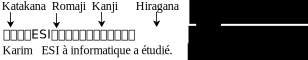
\includegraphics{RATstat/jap-writing.pdf} % % %[width=140mm]
 \caption{Les systèmes d'écriture Japonais.}
 \label{fig:jap-writing}
\end{center}
\end{figure}
%
Pour le Thaï, il comporte moins de caractères avec des mots plus longs que ceux de chinois et de japonais. 
Une bonne segmentation dans cette langue demande une bonne connaissance sur sa lexique et morphologie \cite{96-asanee-al,97-meknavin-al,02-aroonmanakun}.

\subsection{Radicalisation} %Racine du mot
\label{sec:stemming}

Dans tout texte, le même mot pouvait se produire dans des différentes variantes morphologiques. 
Dans la plupart des cas, ces formes lexicales possèdent des interprétations sémantiques similaires, et peuvent être considérées comme équivalentes pour les systèmes de gestion d'information.
Afin que ces systèmes puisent utiliser ces formes comme un seul concept, on utilise souvent un algorithme pour trouver la racine du mot, appelé radicalisateur (\textit{Stemmer}).

La radicalisation tente de réduire un mot vers son radical. 
L'effet n'est pas seulement celui de réduire les différentes variantes d'un terme vers une seule forme représentative, mais aussi de réduire la taille du vocabulaire utilisée par le système pour stocker les représentations. 
Dans la plupart des cas, la petite taille du dictionnaire nous permet de préserver l'espace du stockage et le temps de traitement, ainsi de rendre le document moins bruyant, plus compact, et plus souple \cite{07-hassel}. 

Le résultat d'une radicalisation peut être un mot qui n'a aucun sens, mais qui est commun entre les mots ayant le même sens. 
Le rendement d'une radicalisation dépend sur la racine résultat; il est bon si les différents mots avec le même sens de base ont la même racine, et si les mots qui n'ont pas le même sens sont séparés. 
Selon ces conditions, on peut avoir deux types de problèmes \cite{07-hassel}:
\begin{itemize}
\item Sur-radicalisation: se passe lorsque deux mots sont donnés la même racine, mais en réalité ils ne l'ont pas. 
\item Sous-radicalisation: se passe lorsque les mots qui doivent avoir la même forme de base, ne l'ont pas. 
Par exemple, les deux mots "running" et "ran" doivent avoir la même racine "run", mais le système nous donne "run" et "ran" en ordre.
\end{itemize}

Dans la radicalisation, il existe deux grandes approches \cite{04-brants}: radicalisation linguistique/avec-dictionnaire et radicalisation de style Porter \cite{97-porter}. 
La première méthode donne un meilleur résultat, mais exige un coût d'implémentation et de traitement très élevé pour une petite couverture. 
La deuxième méthode est meilleure de point de vue implémentation et coût de traitement pour une performance acceptable.
Des radicalisateurs ont été développés pour plusieurs langues, ayant compris Malais \cite{00-tai-al}, Latin \cite{96-greengrass-al}, Indonésien \cite{01-sn-bressan}, Suédois \cite{01-carlberger-al}, Néerlandais \cite{96-kraaij-pohlmann}, Allemand \cite{01-monz-rijke}, Français \cite{01-moulinier-al}, Slovène \cite{92-popovic-willett}, Turc \cite{96-ekmekcioglu-al}, et Arabe \cite{02-larkey-al}.

\subsection{Suppression des mots vides}

La suppression de mots vides est une technique commune pour répondre au fait que plusieurs mots dans le document ne contribuent pas particulièrement dans la description de son contenu, et ne font qu'ajouter de bruit. 
La plupart des systèmes de recherche d'information et de résumé automatique, suppriment les mots vides avant de traiter les documents. 
Ceci va augmenter la performance du système, mais éventuellement peut causer des problèmes pour traiter certains cas comme les suivants (les mots vides sont en gras):
\begin{itemize}
\item \textbf{To be or not to be}
\item \textbf{Will and} Grace
\end{itemize}
Pour la première phrase, en supprimant les mots vides, on n'aura aucun mot à traiter, puisque tous les mots sont des mots vides, et donc cette phrase ne participera jamais dans le traitement. 
La deuxième phrase contient le mot "\textit{Will}" qui est un nom, mais le système le considère comme le verbe "\textit{will}" présent dans la liste des mots vides pour l'anglais. 

\section{Critères statistiques}
\label{sec:crit-stat}

Une fois qu'on procède au pré-traitement du texte source, on aura les informations nécessaires pour effectuer le traitement (dans ce cas l'extraction des unités saillantes). 
Pour repérer les unités saillantes (expressions, propositions, phrases, paragraphes) dans le texte, il existe un ensemble de critères statistiques identifiés dans les travaux précédents portant sur le résumé automatique statistique. 

\subsection{Fréquence des mots}

La fréquence des mots (\textit{tf: term frequency}) est le critère le plus utilisé; il a été utilisé par Luhn \cite{58-luhn} pour calculer le score de chaque phrase. 
Il correspond au nombre de fois que la racine d'un mot $ m $ apparaît dans un document $ d $. 
Pour calculer la fréquence d'un mot $ m $, on calcule le nombre d'apparition de toutes ces formes dans le document en question, comme par exemple: "\textit{différencier}", "\textit{différent}", "\textit{différenciation}", etc.
Souvent, le nombre de mots est divisé par le nombre total de mots dans le document, ceci afin de ne pas favoriser les documents longs; ceci peut être représenté par l'équation \ref{eq:tf}.
%
\begin{equation}
\label{eq:tf}
tf(m, d) = \frac{|m|_d}{\sum_{i = 1}^{|d|}{|m_i|_d}}
\end{equation}
Où: 
$ tf(m, d) $ est la fréquence du mot $ m $ dans le document $ d $. 
$ |m|_d $ est le nombre d'occurrences de $ m $ dans le document $ d $. 
$ |d| $ est le nombre de mots différents dans le document $ d $. 

En utilisant la fréquence de mots, on peut rapidement détecter qu'il y a un problème pour les documents du même domaine. 
Dans un domaine donnée, l'informatique par exemple, certains mots sont fréquemment utilisés (exp. ordinateur, informatique, etc.) et donc ces mots vont avoir des grandes fréquences malgré qu'ils ne représentent pas le thème du document. 
Pour contourner ce problème, Salton \cite{73-salton-yang} définit un autre critère appelé $ tf*idf $. 
Le critère $ tf*idf $ exprime qu'un mot est plus important lorsqu'il est plus fréquent dans le document analysé et peu fréquent dans le corpus de documents analysés. 
La propriété $ idf $ s'appelle "\textit{la fréquence inverse de documents}" (en Anglais: \textit{inverse documents frequency}). 
La logique derrière cette propriété est que le mot est plus important lorsqu'il est moins probable de se trouver dans les documents du corpus traité (concernant certain domaine) d'où le mot \textit{inverse} (voir l'équation \ref{eq:idf}).
%
\begin{equation}
\label{eq:idf}
idf(m) = log{\frac{|D|}{|\{d: m \in d\}|+1}}
\end{equation}
Où: 
\begin{itemize}
\item $ |D| $ est le nombre des documents dans le corpus;
\item $ |\{d: m \in d\}| $ est le nombre des documents contenants le mot $ m $.
\end{itemize}
Donc, le facteur $ tf*idf $ va être écrit comme dans l'équation \ref{eq:tf-idf}.
\begin{equation}
\label{eq:tf-idf}
tf*idf(m, d) = tf(m, d)*idf(m)
\end{equation}

\subsection{Position dans le texte}

La position des mots et des phrases dans le texte peut être un bon indicateur de leurs importances. 
Celle-ci peut faire référence à la position de mots dans la phrase \cite{58-luhn}, où bien à la position de la phrase par rapport à une unité (document, section, paragraphe, etc.)\cite{58-baxendale,69-edmundson,97-lin-hovy,04-nobata-sekine}.
%Par exemple, dans les articles scientifiques, l'introduction et la conclusion contiennent des phrases qui résument tous le document. 
Par exemple, dans un paragraphe, les premières et les dernières phrases sont les plus importantes.
Ceci a été prouvé par Baxendale \cite{58-baxendale}, lorsqu'il a utilisé un corpus de 200 paragraphes pour tester l'impact de la position de phrases dans un paragraphe sur son importance. 
Il a trouvé que dans 85\% la première phrase est la plus importante pour le paragraphe, et 7\% pour la dernière. 
Edmundson \cite{69-edmundson}, ensuite, a explicité la position en se basant sur l'hypothèse: "les phrases du thème tendent à apparaître très tôt ou très tard dans un document ou dans ses paragraphes" ("\textit{topic sentences tend to occur very early or very late in a document and its paragraphs}").
Les auteurs de \cite{97-lin-hovy} vont dans le même sens, ils définissent des algorithmes pour l'identification automatique de la position des phrases les plus importantes, mais cette fois en fonction du thème traité.

Dans \cite{04-nobata-sekine}, les auteurs définissent rois méthodes pour le calcul du score de la phrase en utilisant sa position (voir les équations \ref{eq:nobota-pos-1}, \ref{eq:nobota-pos-2}, et \ref{eq:nobota-pos-3}).
%Supposant qu'il y a $ n $ phrases dans le texte d'entrée, pour chaque équation le score de phrase $ p_i $, dont $ i $ est sa position dans le texte, est $ Score_{pos}(p_i) $. 
La première méthode donne $ 1 $ pour les $ N $ premières phrases, et $ 0 $ pour les autres. 
%Sachant que $ N $ est le nombre de phrases dans le résumé.
\begin{equation}
\label{eq:nobota-pos-1}
Score_{pos}(p_i) = \left\lbrace 
\begin{array}{lll}
1 & si & (i<N) \\
0 & sinon & \\
\end{array}
\right. 
\end{equation}
La deuxième méthode suppose que les phrases ont une importance inversement proportionnée à leurs positions. 
\begin{equation}
\label{eq:nobota-pos-2}
Score_{pos}(p_i) = \frac{1}{i}
\end{equation}
La troisième méthode suppose que les phrases dans le début et dans la fin du document sont les plus importantes.
\begin{equation}
\label{eq:nobota-pos-3}
Score_{pos}(p_i) = \max(\frac{1}{i}, \frac{1}{n-i+1})
\end{equation}
Selon les auteurs, la deuxième méthode donne un résultat meilleur que ceux des autres méthodes.

Dans \cite{09-abdelfattah-ren}, les auteurs utilisent la position des phrases dans le paragraphe (et pas dans la totalité de texte). 
Ils supposent que les premières phrases du paragraphe sont les plus importantes, en prenant cinq phrases comme la position maximale (voir l'équation \ref{eq:abdelfattah-pos}). 
\begin{equation}
\label{eq:abdelfattah-pos}
Score_{pos}(p_i) = \left\lbrace 
\begin{array}{lll}
6 - i & si & (i \leq 5)\\
0 & sinon &  \\
\end{array}
\right. 
\end{equation}
Où: $ i $ est la position de phrase dans le paragraphe.

\subsection{Mots du titre et des sous-titres}

Dans \cite{69-edmundson}, l'auteur se base sur l'hypothèse que le titre véhicule le thème du document.
En plus, lorsque l'auteur divise le document en sections, il les résume en leurs choisissant les entêtes (titres de sections) appropriées. 
En suivant cette hypothèse, les phrases importantes sont celles contenant des mots du titre ou des sous-titres.
Bien évidemment, les mots du titre ont plus de poids que ceux des sous-titres.
Dans le travail de \cite{88-salton-buckley}, les auteurs propose d'utiliser le titre comme une requête pour toutes les phrases du document; ensuite la similarité cosinus est calculée entre chaque phrase et le titre. 

%[Ishikawa et al., 2001]
En se basant sur la fréquence de mot, \cite{01-ishikawa-al} proposent une méthode qui prend en considération les mots appartenant au titre. 
En effet, lorsqu'un mot appartient au titre, sa fréquence va être multipliée par un nombre $ A > 1 $. 
Ainsi, le score d'une phrase $ p_i $: $ Score_{titre}(p_i) $ est donné par l'équation \ref{eq:ishikawa-head}.
\begin{equation}
\label{eq:ishikawa-head}
Score_{titre}(p_i) = \sum_{\{m\} \in p_i}{\alpha(m) * tf(m)}
\end{equation}
Où: 
\begin{equation}
\label{eq:ishikawa-head2}
\alpha(w) = \left\lbrace 
\begin{array}{lll}
A > 1 & si & w \in Titre \\
1 & sinon & \\
\end{array} 
\right. 
\end{equation}

%04-nobata-sekine
Dans \cite{04-nobata-sekine}, deux méthodes sont utilisées pour calculer le score des phrases en se basant sur les mots du titre. 
Pour chaque phrase $ p_i $ et sachant le titre $ T $,  le score de cette phrase est donné par $ Score_{titre}(p_i) $. 
La première méthode utilise le $ tf*idf $ des mots de titre, comme il est indiqué dans l'équation \ref{eq:nobta-head-1}.
\begin{equation}
\label{eq:nobta-head-1}
Score_{titre}(p_i) = \frac{\sum_{m \in T \bigcap p_i}{\frac{tf(m)}{tf(m)+1} idf(m)}}
{\sum_{m \in T}{\frac{tf(m)}{tf(m)+1} idf(m)}}
\end{equation}
La deuxième méthode utilise les entités nommées et la fréquence de mots $ tf $. 
Pour une entité nommé $ e $, l'équation \ref{eq:nobta-head-2} est utilisée pour calculer le score d'une phrase $ p_i $ en se basant sur le titre.
\begin{equation}
\label{eq:nobta-head-2}
Score_{titre}(p_i) = \frac{\sum_{e \in T \bigcap p_i}{\frac{tf(e)}{tf(e)+1}}}
{\sum_{e \in T}{\frac{tf(e)}{tf(e)+1}}}
\end{equation}
Selon les auteurs, la deuxième méthode donne un meilleur résultat. 

\subsection{Longueur de phrase}

Ce critère est utilisé pour pénaliser les phrases qui sont trop petites, vu que ces phrases ne serons pas incluses dans le résumé \cite{95-kupiec-al}. 
Le score pour ce critère est la longueur normalisée de phrase; qui est la proportion entre le nombre de mots dans la phrase et le nombre de mots dans la phrase la plus longue dans le document \cite{02-neto-al,04-nobata-sekine}.

Dans le travail de \cite{04-nobata-sekine}, deux méthodes sont utilisées. 
La première donne un score égale au longueur de phrase divisée par une longueur $ L_{max} $ prédéfinie, si la longueur de phrase est supérieure à $ L_{max} $ on lui attribue un score égale à $ 1 $ (voir l'équation \ref{eq:nobota-len-1}). 
\begin{equation}
\label{eq:nobota-len-1}
Score_{long}(p_i) = \left\lbrace 
\begin{array}{lll}
\frac{L_i}{L_{max}} & si & (L_i \leq L_{max}) \\
1 & sinon & \\
\end{array}
\right. 
\end{equation}
La deuxième méthode donne un score négatif afin de pénaliser les phrases qui sont plus courtes que $ L_{min} $ (voir l'équation \ref{eq:nobota-len-2}). 
\begin{equation}
\label{eq:nobota-len-2}
Score_{long}(p_i) = \left\lbrace 
\begin{array}{lll}
0 & si & (L_i \geq L_{min}) \\
\frac{L_i - L_{min}}{L_{min}} & sinon & \\
\end{array}
\right. 
\end{equation}
Selon les auteurs, la deuxième méthode donne un meilleur résultat. 

Une autre formule pour calculer le score d'une phrase $ p_i $ dans un document $ d $ en utilisant sa longueur, est utilisée dans \cite{09-abdelfattah-ren} (voir l'équation \ref{eq:abdelfattah-len}). 
\begin{equation}
\label{eq:abdelfattah-len}
Score_{pos}(p_i) = \frac{|p_i| * |\{P: P \in d\}|}{|d|}
\end{equation}
Où: 
$ |p_i| $ et $ |d| $ sont les nombres de mots dans la phrase $ p_i $ et le document $ d $ respectivement. 
$ |\{P: P \in d\}| $ est le nombre de phrases dans le document $ d $. 

\subsection{Mots indicatifs} % indicatifs clés
%the presence of cue words and expressions such as “important”, “definitely”,  “in particular” (all positive), and “unclear”, “perhaps”, “for example” (all negative) [Edmundson 1969; Rush et al. 1971]; (93-paice-jones)

Les méthodes utilisant les mots indicatifs (\textit{cue words}), sont basées sur l'hypothèse que la pertinence d'une phrase est affectée par la présence de mots comme "\textit{significatif}", "\textit{impossible}", et "\textit{difficilement}" \cite{69-edmundson}. 
Ces méthodes utilisent des mots sauvegardés dans un dictionnaire extrait à partir d'un corpus. 
Le dictionnaire de mots clés contient trois sous-dictionnaires: Les mots \textit{Bonus}, qui sont pertinents positivement (\textit{important}, \textit{précisément}, \textit{particulièrement}, etc.); Les mots \textit{Stigmates}, qui sont plutôt pénalisant (\textit{obscurément}, \textit{peut-être}, etc.); et les mots \textit{Null}, qui ne sont pas indicatifs. 
Le score total pour une phrase $ p_i $ basé sur ce critère, est la somme des poids $ cue(m) $ pour ses mots constituants $ m $. 
Ceci est indiqué dans l'équation \ref{eq:edmundson-cue}, où $ cue(m) $ est le poids du mot $ m $ par rapport au dictionnaire de mots clés. 
\begin{equation}
\label{eq:edmundson-cue}
Score_{cue}(p_i) = \sum_{m \in p_i}{cue(m)}
\end{equation}
Sachant que:
\begin{equation}
\label{eq:edmundson-cue2}
cue(m) = \left\lbrace 
\begin{array}{lll}
b > 0 & si & (w \in Bonus) \\
\delta < 0 & si & (w \in Stigma) \\
0 & sinon & 
\end{array} 
\right. 
\end{equation}

Dans \cite{09-abdelfattah-ren}, les mots clés positifs sont définis par "les mots fréquemment inclus dans le résumé". 
Le score d'une phrase $ p_i $ en utilisant les mots clés positifs, est donné par l'équation \ref{eq:abdelfattah-cue+}. 
\begin{equation}
\label{eq:abdelfattah-cue+}
Score_{cue}(p_i) = \frac{1}{|p_i|} \sum_{m \in p_i}{tf(m) * P(p_i \in R | m)}
\end{equation}
Où: 
$ P(p_i \in R | m) $ est la probabilité que la phrase $ p_i $ appartienne au résumé $ R $ sachant qu'elle contient le mot $ m $. 
Cette probabilité peut être calculée en utilisant un corpus d'apprentissage (contenant des résumés modèles), et en appliquant l'équation \ref{eq:abdelfattah-prob}. 
\begin{equation}
\label{eq:abdelfattah-prob}
P(p_i \in R | m) = \frac{P(m | p_i \in R) * P(p_i \in R)}{P(m)}
\end{equation}
Par conséquent, les mots clés négatifs sont les mots peu probables d'être dans un résumé (voir l'équation \ref{eq:abdelfattah-cue-})
\begin{equation}
\label{eq:abdelfattah-cue-}
Score_{cue}(p_i) = \frac{1}{|p_i|} \sum_{m \in p_i}{tf(m) * P(p_i \notin R | m)}
\end{equation}

\subsection{Expressions saillantes}
%These are commonly occurring structures which explicitly state that the sentences containing them have something important to say about the subject matter or the 'message' of the document. 

Les expressions saillantes sont des structures, lorsqu'elles se produisent dans une phrase, expriment explicitement que cette phrase contient une information importante à propos du sujet ou un "message" du document \cite{81-paice}. 
Par exemple "\textit{Le but principal de cet article est de vérifier ...}", "\textit{Dans cet article, une méthode est décrite pour ...}", etc.
D'après Paice, l'identification des expressions saillantes n'est pas une tâche simple (une comparaison de chaînes de caractères ne suffit pas), à cause des raisons suivantes:
\begin{itemize}
\item On ne peut pas lister toutes les expressions saillantes à cause des variations qui peuvent exister. 
Par exemple, les expressions suivantes ont la même structure: "\textit{This article is concerned with ...}", "\textit{Our paper deals with ...}", "\textit{The present report concerns ...}" et "\textit{The following discussion is about ...}". 
Donc, la solution est d'utiliser des modèles contenant des mots appelés \textit{les paradigmes} (prototypes, modèles). 

\item En utilisant les modèles, il parait qu'il existe des mots qui ne figurent pas dans ces modèles malgré qu'ils fassent partie d'une expression indicative. 
La solution est d'utiliser des sauts limités entre les paradigmes d'un modèle donné.

\item Il existe des mots qui sont optionnels, mais qui ajoute un poids lorsqu'on les utilise, comme le mot "\textit{here}" dans l'expression "\textit{The purpose \textbf{here} is to ...}". 
On peut définir de multiples chemins dans le modèle. 

\item Enfin, les mots peuvent avoir plusieurs variations, ce problème peut être résolu en utilisant leurs racines dans les modèles. 
\end{itemize}
La figure \ref{fig:paice-template} représente un modèle pour détecter les expressions saillantes, où les mots sont les paradigmes. 
Les limites de sauts entre les paradigmes sont présentées comme [3]. 
Le gain de poids de l'expression est présenté comme +2. 
Les paradigmes suivis par (?) sont optionnels.
%
\begin{figure}[ht]
\begin{center}
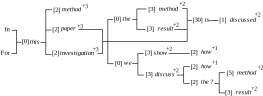
\includegraphics{RATstat/paice-template.pdf} % % %[width=140mm]
 \caption[Un des modèles pour détecter les expressions saillantes] %
 {Un des modèles pour détecter les expressions saillantes (version simplifiée) \cite{81-paice}.}
 \label{fig:paice-template}
\end{center}
\end{figure}

\subsection{Combinaison des critères}

Tous ou une partie des critères précédemment présentés sont combinés sous forme d'une combinaison linéaire en les attribuant un poids à chaque critère (voir l'équation \ref{eq:combin-crit}).
\begin{equation}
\label{eq:combin-crit}
Score(p_i) = \sum_{c \in Criteres}{\alpha_c * Score_c(p_i)}
\end{equation}
Pour un poids $ \alpha_c $ d'un critère $ c $, la définition de la valeur était manuelle ou intuitive, dans les premiers travaux de résumé automatique. 
Dans \cite{69-edmundson}, l'auteur utilise quatre critères: les mots indicatifs (\textit{C: Cue}), la fréquence de mots (\textit{K: Key}), les mots de titre (\textit{T: Title}), et la position (\textit{L: Location}). 
Les quatre critères précédents sont combinés pour calculer le score de la phrase ($ S = \alpha_lC + \alpha_2K + \alpha_3T + \alpha_4L $), ce qui nous donne 15 combinaisons différentes. 
La figure~\ref{fig:edmundson-score} représente le pourcentage moyen de pertinence des combinaisons les plus intéressantes, ainsi que l'intervalle entre le pourcentage moyen moins et plus l'écart standard.
%with the intervals encompassing the sample mean plus and minus one sample standard deviation. 
%
\begin{figure}[ht]
\begin{center}
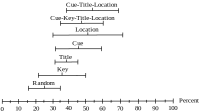
\includegraphics{RATstat/edmundson-score.pdf} % % %[width=140mm]
 \caption[Les moyennes des scores de pertinence pour chaque combinaison de critères]{Les moyennes des scores de pertinence pour chaque combinaison de critères \cite{69-edmundson}.}
 \label{fig:edmundson-score}
\end{center}
\end{figure}
Avec l'avènement des techniques d'apprentissages, ces derniers ont été utilisés dans le but d'estimer les poids de critères (voir la section~\ref{sec:appentissage}). 
%Plusieurs techniques d'apprentissage ont été utilisés: les algorithme génétiques, la régression mathématique, réseau de neurone \cite{09-abdelfattah-ren}.

\section{Amélioration de l'approche statistique}

Le choix de différents poids pour chaque critère est difficile, puisque chaque genre de document se base sur des critères spécifiques plus que d'autres. 
Par exemple, dans un document de presse, le critère de position est très important puisque l'information pertinente se trouve au début, donc il faut donner un poids élevé à ce critère pour ce genre de documents. 
Une autre limite est le manque de ressources linguistiques en plus du bruit introduit par la considération de la totalité des phrases pour ne garder que l'information pertinente.
C'est pourquoi plusieurs recherches ont été menées afin d'améliorer l'approche statistique.

\subsection{Techniques linguistiques}

Il existent des travaux qui intègrent des données linguistiques avec l'approche statistique, notamment en utilisant les graphes de similarité \cite{02-neto-al,09-abdelfattah-ren}, ou en utilisant les parties du discours (\textit{part of speech})\cite{96-kraaij-pohlmann,02-neto-al}, etc.
Après l'application de ces techniques, on obtient des propriétés linguistiques qui peuvent être traitées statistiquement en comptant leurs fréquences, par exemple le nombre de noms dans une phrase.

La cohésion entre les phrases est une propriété importante.
En effet, plus un résumé contient des phrases liées, plus sa qualité augmente. 
Dans cette logique, \cite{09-abdelfattah-ren} utilise le nombre des arcs dans le graphe de similarité de toutes les phrases, pour calculer l'importance d'une phrase. 
L'équation \ref{eq:abdelfattah-arcs} représente le score de ce critère, où $ G =  \{S, A\} $ est le graphe de similarité entre les phrases, $ S $ est l'ensemble de sommets (phrases), et $ A $ est l'ensemble des arcs.
\begin{equation}
\label{eq:abdelfattah-arcs}
Score_{\#arcs}(p_i) = |\{ p_j : a(p_i, p_j) \in A / p_j \in S, p_i \neq p_j \}|
\end{equation}

Dans \cite{02-neto-al}, les auteurs utilisent la somme des poids (de similarité) des arcs reliant la phrase avec le reste des phrases. 
Supposant que $ W(x, y) $ est le poids de l'arc liant $ x $ à $ y $, i.e. la similarité entre les phrases $ x $ et $ y $, le score de ce critère est donné par l'équation \ref{eq:arcs-weight}.
\begin{equation}
\label{eq:arcs-weight}
Score_{poids-arcs}(p_i) = \sum_{p_j \in S} W(p_i, p_j) / a(p_i, p_j) \in A , p_i \neq p_j
\end{equation}

Un autre traitement linguistique qui a prouvé son utilité pour le résumé automatique (et la recherche d'information) est l'intégration des parties de discours. 
Dans \cite{96-kraaij-pohlmann}, des expériences sont faites pour vérifier l'effet des différentes parties de discours sur la recherche d'information, en les utilisant comme des termes de requête. 
Pour le Néerlandais, ils trouvent que 58\% des termes réussis sont des noms, 29\% sont des verbes, 13\% sont des adjectifs. 
Dans le résumé automatique, l'occurrence des noms propres est utilisée par \cite{02-neto-al} comme critère. 
Ceci est motivé par le fait que les noms propres, qui font référence à des gens ou des places, sont des indices que la phrase est pertinente pour le résumé.
Dans ce travail, on considère seulement la présence ou non de noms propres et pas leurs nombres. 

\subsection{Apprentissage}
\label{sec:appentissage}

L'objectif principal de tout algorithme d'apprentissage automatique est d'apprendre, d'identifier un ensemble de règles depuis un corpus de documents, ces règles sont ensuite appliquées sur le ou les textes en entrée du système de résumé. 
Dans ce type de systèmes, on définit deux principales phases  qui sont:  la phase d'entraînement et la phase de tests. 
Dans la première phase, l'ensemble des caractéristiques sont extraites du corpus d'entraînement pour générer, ensuite, des règles de classification en utilisant un algorithme d'apprentissage.
Dans la deuxième phase, ces règles sont appliquées sur le corpus de test afin de générer les résumés correspondants. 
Tous les travaux précédents suivent les mêmes phases, la différence réside dans le choix de l'algorithme d'apprentissage le plus approprié \cite{95-kupiec-al,02-osborne,05-yeh-al}, le traitement des problèmes liés à la phase d'entraînement tels que l'absence ou la taille réduite des corpus étiquetés \cite{01-amini-gallinari}, la combinaison des critères hétérogènes \cite{08-wong-al,10-yatsko-al}, etc. 

Étant donné un corpus qui contient des documents avec leurs résumés extractifs, on peut utiliser un algorithme d'apprentissage pour estimer qu'une phrase appartient au résumé ou non. 
Les auteurs de \cite{95-kupiec-al} proposent un système de résumé par apprentissage basé sur la classification de Bayes, afin de calculer la probabilité qu'une phrase appartient au résumé, pour enfin réorganiser les phrases selon leurs probabilités et extraire les premières. 
Ainsi, pour chaque phrase $ p_i $, on calcule la probabilité qu'elle peut être sélectionnée dans un résumé $ R $ étant donné le vecteur de critères $ \overrightarrow{f} $ (l'équation \ref{eq:bayes-kupiec}).
\begin{equation}
\label{eq:bayes-kupiec}
P(s_i \in R | \overrightarrow{f}) = %
\frac{\prod_{j = 1}^{|\overrightarrow{f}|} P(f_j | s_i \in R) . P(s_i \in R)}
{\prod_{j = 1}^{|\overrightarrow{f}|} P(f_j)}
\end{equation}
Où: 
$ P(s_i \in R) $ est une constante, et les deux probabilités $ P(f_j | s_i \in R) $ et $ P(f_j) $ peuvent être estimées de corpus d'entrainement en calculant les occurrences.

Le problème majeur avec l'utilisation d'un classificateur bayésien est l'indépendance supposée de critères, Osborne a tenté de résoudre ce problème en utilisant un modèle logarithmique linéaire \cite{02-osborne}. 
L'utilisation de classificateur basé sur le principe du maximum d'entropie (Maxent) donne une performance au-dessous du classificateur Na\"ive-Bayes, mais le surpasse lorsqu'on utilise une probabilité à priori avec Maxent. 
Dans sa version, au lieu de réorganiser les phrases en utilisant leurs probabilités, Osborne utilise un algorithme d'apprentissage pour classifier les phrases dans deux classes: la première contient les phrases de résumé, et la deuxième contient les autres phrases. 

\cite{01-amini-gallinari} tentent d'atténuer les problèmes causés par l'absence de corpus étiquetés, en proposant une méthode auto-supervisée. %; qui ne se base pas sur la disponibilité des corpus libellés pour l'apprentissage. 
Le modèle proposé peut être utilisé dans les résumés généraux, ainsi que dans les résumés par requête. 

Contrairement aux travaux précédents, \cite{05-yeh-al} proposent une méthode qui, au lieu de trouver la probabilité ou la classe d'une phrase, attribue des poids aux critères utilisés en utilisant un corpus d'apprentissage. 
Pour ce faire, ils utilisent un algorithme génétique pour attribuer ces poids (la position de phrase, les mots clés, le centre, et la similarité avec le titre). 
Le score final d'une phrase est la somme des scores de chaque critère multiplié par son poids.

De même, \cite{08-wong-al} proposent une approche par apprentissage afin de combiner des critères hétérogènes. 
Ces critères sont classés en quatre catégories: surface, contenu, pertinence, et événement. 
Les critères de surface sont ceux qui se basent sur les aspects extrinsèques d'une phrase: la position de phrase, la longueur de phrase, etc. 
Les critères de contenu mesurent le score d'une phrase sur la base des mots la composant: les fréquences de mots dans le document.
Les critères de pertinence évaluent la relation d'une phrase avec les autres: la similarité par rapport à la première phrase du document. 
Les critères d'événement représentent les phrases par leurs événements: les verbes et les noms qui comportent des actions.

Dans \cite{10-yatsko-al}, les auteurs vont plus loin et proposent d'utiliser 45 paramètres de différents types : statistiques, de positionnement et discursives afin d'identifier celles qui sont les plus pertinentes pour un genre de document donné (scientifique, presse, et artistique).
En utilisant un algorithme de regroupement (K-Means), ils ont regroupé les documents d'un corpus selon les genres précédents. 
Ensuite, le corpus est utilisé pour identifier les paramètres spécifiques pour chaque genre en attribuant à chacun un poids. 

\subsection{Compression de phrases}

Souvent, les résumés automatiques par extraction contiennent des informations superflues, ceci arrive surtout lorsque le résumé contient des phrases très longues. 
La compression des phrases élimine les parties non nécessaires, et produit des résumés plus abrégés et plus précis. 
Dans \cite{99-jing-mckeown}, les auteurs affirment que la compression de phrases est souvent utilisée par les résumeurs professionnels. 
En effet, on a trouvé que 78\% des phrases de résumé ont été reprises du document d'entrée, et plus de la moitié ont fait l'objet de compression.

Il existe deux approches pour la compression de phrases: la première utilise des techniques linguistiques primitives, et la dernière utilise des techniques statistiques. 
La première utilise des règles syntaxiques et du discours pour déterminer la manière de compression d'une phrase. 
Les règles syntaxiques consistent à la définition de la structure syntaxique de la phrase: son arbre syntaxique ainsi que les constituants à enlever; i.e. ceux avec une faible probabilité.
%La connaissance syntaxique contient la structure syntaxique d'une phrase, et les constituants les moins probables d'être dans le résumé. 
Bien que La connaissance du discours contienne l'information des différentes connections des constituants dans le résumé. 
%
\cite{00-jing} propose un système de compression de phrases, qui utilise de multiples sources de connaissance pour décider quelle expression à éliminer de la phrase extraite. 
Ces sources comportent l'information syntaxique, l'information contextuelle, et des statistiques extraites d'un corpus de résumés professionnels. 
%
Dans le travail de \cite{07-Zajic-al}, la compression des phrases se fait avant leur extraction, et la suppression des constituants se fait intuitivement. 
La compression est exécutée itérativement en supprimant un constituant à la fois. 
À chaque itération la sortie constitue l'entrée d'un module d'extraction, ce dernier utilise six critères pour calculer le score de la phrase.

Dans la deuxième approche, l'approche statistique, les règles de suppression des constituants syntaxique sont apprises par programme, et donc aucune règle linguistique ne doit être fournie comme entrée. 
%
Dans \cite{02-knight-marcu}, deux méthodes basées sur l'approche statistique sont développées: en utilisant le modèle de canal bruyant (\textit{the noisy channel model}), et les arbres de décision. 
Dans la première méthode, l'idée est de supposer que la phrase d'entrée du modèle était courte, qui a été modifiée avec d'autres mots additionnels, d'une manière ou d'une autre.
Étant donnée une phrase longue, le programme produit un arbre syntaxique et émet les différentes hypothèses pour réduire cet arbre. 
Ils mesurent la qualité des arbres en utilisant les scores de \textit{probabilistic context free grammar (PCFG) } et les probabilités de phrase suivant le modèle du langage bi-gramme. 
Ils mesurent la vraisemblance de la transformation d'un arbre large vers un arbre réduit en utilisant des statistiques rassemblés d'un corpus contenant des documents avec leurs résumés. 
La deuxième méthode se base sur les arbres de décision qui sont utilisées pour apprendre les différentes règles appliquées pour réduire les phrases.
%
%Galley and McKeown [65] make two
%significant improvements. They move to a lexicalized head-driven
%approach that allows them to take the lexical heads of constituents
%into account before making deletions. This helps them to avoid deleting
%negation words such as “no” and “not”, which would completely change
%the meaning of the sentence, a problem which Knight and Marcu’s
%approach cannot handle. 

D'autres méthodes ont été proposées pour améliorer la compression de phrases, en utilisant non seulement une seule phrase mais en utilisant les autres qui lui ressembles.
Dans le travail de \cite{08-cohn-lapata}, la tâche de compression de phrases est généralisée.  
Au lieu de raccourcir la phrase en éliminant des mots ou des constituants, ils introduisent des opérations additionnelles comme la substitution, la ré-ordonnancement, et l'insertion.
Dans \cite{10-filippova}, une méthode est développée pour résumer un groupe de phrases reliées avec une phrase plus réduite. 
Dans cette méthode, les phrases sont représentées par un seul graphe, et en prenant le plus court chemin, on obtient un résumé réduit.

\section{Post-traitement}

Dans l'approche statistique, la présentation du résumé est un problème.
En effet, les phrases extraites sont des phrases dispersées au long du texte source, et qui n'ont à priori aucune relation directe. 
Le premier problème à résoudre est la manière dont on organise les phrases extraites pour avoir un résumé cohérent. 
Le deuxième étant l'existence des anaphores dans le résumé.

\subsection{Ordonnancement des phrases} %Assemblage des phrases
%/home/karim/Compression/Nenkova_Overview.pdf

Pour assembler les différentes phrases extraites, il faut d'abord définir leur ordre. 
Cette opération a un impact direct sur la qualité de résumé; un résumé avec des phrases désordonnées est difficile à lire et à comprendre. 
Dans le résumé mono-document, la solution était de préserver l'ordre des phrases dans le document d'origine \cite{99-mckeown-al,00-radev-al,02-lin-hovy}. 
Malgré que, en observant les résumés professionnels, on peut trouver que les phrases ne préservent pas leurs ordres initiaux. 
Dans le résumé multi-document, la tâche est encore plus difficile, puisque l'entrée consiste à plusieurs documents avec des thèmes non nécessairement abordés dans tous ces documents. 
En plus, même pour les phrases des thèmes communs, ces thèmes n'ont pas nécessairement le même ordre dans les documents d'entrée. 

Une des solutions proposées pour le résumé multi-documents est l'ordre de majorité (\textit{Majority Ordering}) \cite{02-barzilay-al}. 
Dans cette solution, on regroupe les phrases similaires provenant de différents documents. 
Ensuite, un graphe qui représente l'ordre local dans l'entrée est construit, où chaque sommet représente un thème. 
Deux sommets sont connectés par un arc, si dans un document, une phrase d'un thème est immédiatement suivie par celle du deuxième thème. 
Le poids de l'arc est le nombre des articles où cet ordre est observé. 
Pour inférer l'ordre global de graphe, un algorithme d'approximation est utilisé. 
Des variations de cette méthode ont été étudiées par plusieurs travaux \cite{05-bollegala-al,08-ji-nie}.

\cite{08-boudin-al} définissent un ensemble d'opérations où différentes expressions sont réécrites à leurs formes standards (acronymes, dates et nombres, références temporelles), les outils de jonction entre les phrases sont éliminés (l'expression "\textit{But, it is ...}" devient "\textit{It is ...}"), ainsi que le contenu parenthésé. 

\subsection{Résolution des anaphores}

Dans le résumé par extraction, les phrases extraites pourraient contenir des références anaphoriques non résolues.
Par exemple, supposant qu'on a le texte suivant:
\begin{quote}
"\textit{\textbf{Cosette} était à sa place ordinaire, assise sur la traverse de la table de cuisine près de la cheminée. 
\textbf{Elle} était en haillons, \textbf{elle} avait ses pieds nus dans des sabots, et elle tricotait à la lueur du feu des bas de laine destinés aux petites Thénardier.}"\footnote{Extrait de livre "LES MISÉRABLES - Tome II - COSETTE" par Victor Hugo (1862)}
\end{quote}
Si le résumé contient uniquement la deuxième phrase, on perd la référence "\textbf{Elle}", et donc ça va diminuer la qualité du résumé. 
C'est pourquoi, il faut récupérer la référence de ce pronom, et le remplacer par cette référence, mais le deuxième pronom dans la phrase doit rester tel qu'il est.

Parmi les premiers travaux de résolution automatique des anaphores, on peut citer celui de \cite{78-hobbs}. 
Sa méthode effectue une analyse syntaxique suivie par l'établissement des chaînes de référence en parcourant l'arbre syntaxique suivant un certain ordre. 
La sélection d'un antécédent se fait en utilisant des critères de compatibilité syntaxique et sémantique (genre, nombre, animation...) avec l'élément anaphorique. 
De même, les auteurs de \cite{94-lappin-leass} développent une méthode semblable pour la résolution automatique des anaphores. 
Mais, plutôt que de parcourir un arbre syntaxique selon un ordre particulier, des scores sont attribués aux candidats antécédents, selon un ensemble de caractéristiques (distance, fonction syntaxique, construction existentielle).

Afin de diminuer l'utilisation de ressources linguistiques, nécessaires pour les travaux précédents, d'autres travaux adoptent une approche \textit{knowledge-poor}.
Parmi ces travaux, on trouve le travail de \cite{98-mitkov}, où on propose un algorithme qui identifie les syntagmes référentiels, et valorise les syntagmes définis, le thème de la phrase, les réitérations lexicales et l'appartenance de la tête nominale au vocabulaire du domaine ou aux mots du titre, afin de sélectionner l'antécédent. 
Dans \cite{97-baldwin}, on remarque que les antécédents se situent habituellement dans la phrase courante ou la phrase précédente.

Aujourd'hui, il existe des outils pour la résolution des anaphores, qu'on peut utiliser dans les systèmes de résumé automatique. 
Parmi ces outils, JavaRAP \cite{04-qiu-al}, qui résout les pronoms de la troisième personne, les anaphores lexicales, et identifie les pronoms pléonastique (le pronom "\textit{it}" souvent utilisé sans référence à quelque chose: "\textit{it is important to \ldots}").

\section{Conclusion}

Dans ce chapitre, nous avons présenté un état de l'art sur le résumé automatique de texte basé sur l'approche statistique. 
Dans un premier temps, nous avons présenté un des premiers travaux dans le domaine, celui de Luhn \cite{58-luhn}, comme illustration du principe de fonctionnement de tels systèmes.
Ainsi, nous avons présenté l'étape de pré-traitement constituée d plusieurs opérations (normalisation, segmentation, etc.), ceci pour avoir une entrée standard au module de résumé. 
Ensuite, nous avons présenté quelques critères utilisés pour le calcul des scores de phrases dans l'approche statistique: la fréquence de mots, la position, mots de titre, la longueur, les mots indicatifs,  et les expressions indicatives. 
Ces différents critères sont combinées pour avoir un seul score, égale à la somme des scores de chacun multiplié par son poids. 
Nous avons discuté des méthodes pour l'améliorer en utilisant des outils linguistiques, par apprentissage, et par compression de phrases. 
Le résumé produit nécessite encore des améliorations du point de vu fluidité de lecture et de compréhension. 
Donc, une étape de post-traitement est nécessaire pour résoudre, ou au moins diminuer l'effet de ces problèmes. 
C'est pourquoi nous avons discuté l'ordonnancement des phrases et la résolution des anaphores. 

Le résumé par approche statistique prend sa puissance des techniques de recherche d'information, avec l'avantage de traiter les documents en général indépendamment à leurs genres, langues, etc. 
Cette approche a prouvé son utilité pour la recherche d'information, en prenant les unités les plus pertinentes décrivant le thème de document, l'indexation devient donc plus facile.
Mais, lorsqu'on veut générer un résumé professionnel, cela va nous conduire à se poser des questions sur la présentation du résumé. 
Ainsi, le modèle de sac de mots de la RI n'est plus suffisant et le besoin d'outils linguistiques est nécessaire à un certain niveau.

Dans le chapitre suivant, nous allons présenter les différentes méthodes d'évaluation de résumé automatique de textes.

%========================Le pied de chapitre=======================================
%==================================================================================
\ifx\wholebook\relax\else
 \cleardoublepage
 \bibliographystyle{../use/ESIbib}
 \bibliography{../bib/RATstat}
 \end{document}
\fi
%==================================================================================